\chapter{Results}
\label{chap:results}

\section{Current Evidence and Correctness}
\label{sec:results-correctness}

The current matched experiments completed at source \texttt{4a83fa6}, whose
Python sources are identical to calibration source \texttt{c5b5ac3}. The
common and targeted datasets remain separate. Both archives passed independent
reconstruction of inputs, configuration, schedule, outputs, frozen batch sizes
and statistics. An additional analysis rebuilt the per-input medians and
quartiles from every original sample record and matched the validator's values.
The manifest-bound records and reproducible analysis are indexed in
\cref{sec:appendix-current-formal}.

\begin{table}[htbp]
\centering
\caption{Current formal execution. Calls within a batch are not independent samples.}
\label{tab:results-current-counts}
\begin{tabular}{lrrrr}
\toprule
Dataset & Inputs & Sample batches & Sample calls & Warm-up calls\\
\midrule
Common & 140 & 5600 & 62720 & 1400\\
Targeted split & 12 & 480 & 3840 & 120\\
\bottomrule
\end{tabular}
\end{table}

Each input/backend contributes twenty sample batches after five warm-up calls.
All 66,560 sample calls and 1,520 warm-up calls returned the expected output;
no case was erroneous, timed out, skipped or replaced. This output observation
is separate from the previously established v2 qualification: formal timing
does not repeat checked audits inside the timer. Neither repeated calls nor
related constructions create additional independent inputs, and the observed
success is finite evidence rather than the general correctness argument.

\section{Common-Set Runtime and Paired Ratios}
\label{sec:results-runtime-size}
\label{sec:results-ratios}

The runs use Apple M4/arm64, 16 GB RAM, ten logical CPUs, macOS 26.6 and
CPython 3.12.14, with GC enabled at thresholds 700/10/10. The captured power
state is battery power at 100\%; the records do not establish constant clock
frequency or thermal state throughout execution. Both backends use the same
public minimal sorting scope, and the tree disables detailed work collection while retaining access hooks
(\cref{sec:implementation-policies}).
Initialization, sorting, output recovery, the batch loop and output append are
included; expected-output comparisons and persistence are excluded.

\Cref{tab:results-runtime-size} gives medians across input-specific medians.
The last column is instead the median of ratios formed within each input;
it is not obtained by dividing the two aggregate time columns. Ratios above
one mean a slower tree implementation under this protocol.

\begin{table}[htbp]
\centering
\caption{Common set: descriptive runtime and matched ratios. Times are milliseconds per call; each input first contributes a median of twenty batch-derived observations.}
\label{tab:results-runtime-size}
\begin{tabular}{rrrrr}
\toprule
$n$ & Inputs & List (ms) & Tree (ms) & Median ratio\\
\midrule
    32 & 14 & 0.612 & 1.934 & 3.153 \\
    33 & 14 & 0.620 & 1.957 & 3.086 \\
    64 & 14 & 1.291 & 3.646 & 3.030 \\
    65 & 14 & 1.275 & 4.012 & 3.089 \\
    128 & 14 & 2.642 & 8.082 & 2.898 \\
    129 & 14 & 2.772 & 8.002 & 2.890 \\
    256 & 14 & 6.146 & 13.999 & 2.625 \\
    257 & 14 & 6.218 & 15.427 & 2.600 \\
    512 & 14 & 16.390 & 29.041 & 2.098 \\
    513 & 14 & 16.136 & 33.791 & 2.123 \\
\bottomrule
\end{tabular}
\end{table}

\begin{figure}[htbp]
\centering
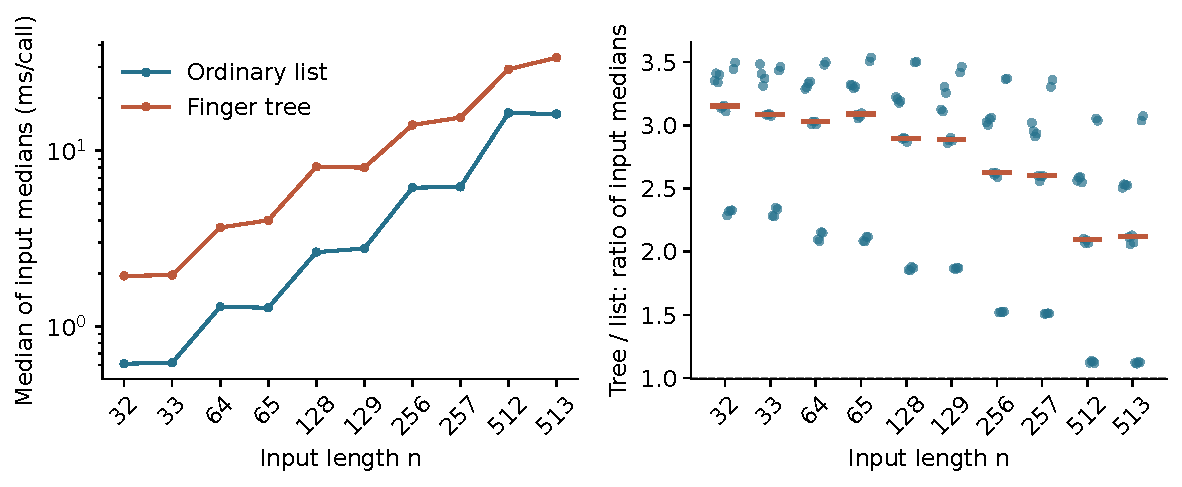
\includegraphics[width=\textwidth]{current_formal_common.pdf}
\caption{Current common set. Left: medians of input medians, with a logarithmic time axis. Right: all fourteen input ratios per length; horizontal marks are their medians. Horizontal offsets only separate points. The dashed line denotes equal runtime, not a confidence bound.}
\label{fig:results-runtime-size}
\end{figure}

Across the 140 inputs, tree/list ratios range from 1.114 to 3.535, with
median 2.898 and cross-input quartiles 2.117 and 3.210. Every input has a tree
median above its matched list median. The size-stratum median decreases from
3.153 at $n=32$ to 2.123 at $n=513$, with local nonmonotonic changes. This
narrowing gap does not establish a future crossover; no crossover was observed.

\subsection{Structural Strata}
\label{sec:results-family}

\begin{table}[htbp]
\centering
\caption{Common-set ratios grouped by the frozen nesting classification. These aggregates mix lengths and related constructions. Split counts are per backend in qualification traces.}
\label{tab:results-family-ratios}
\begin{tabular}{lrrrr}
\toprule
Stratum & Inputs & Median ratio & Range & Two-sided splits\\
\midrule
Strict-flat & 20 & 3.439 & 3.035--3.535 & 0\\
Low nesting & 40 & 3.198 & 2.505--3.484 & 0\\
Medium nesting & 40 & 2.886 & 2.058--3.157 & 0\\
Heavy nesting & 40 & 1.868 & 1.114--2.348 & 0\\
\bottomrule
\end{tabular}
\end{table}

The heavy group has the smallest descriptive ratios, but this is not a causal
estimate of nesting cost. Constructors change more than one feature and mirror
pairs are dependent. In particular, the qualification traces contain 3,788
split calls per backend but no two-sided splits: all take an empty-side
outcome. Those executions cover insertion, whole-group movement and ownership
updates, not the interior search/dismantle/join path. A nesting label must not
be interpreted as a split-work label.

\section{Independent Targeted Split Set}
\label{sec:results-targeted}

The twelve targeted inputs at $n=128,129$ contain the intended nonempty
splits: the smaller side is 3, 7 or 19, each represented by four inputs.
Source size is 61 under a finite owner. The traces also cover subsequent
retained-side insertion, but not updates to both outputs in every case.
Those facts come from qualification traces; formal minimal runs do not collect
an intrusive detailed operation ledger.

\begin{table}[htbp]
\centering
\caption{Targeted set, separately analyzed. Each $k$ group has both lengths and both directions.}
\label{tab:results-targeted}
\begin{tabular}{rrrrr}
\toprule
$k$ & Inputs & List (ms) & Tree (ms) & Median ratio\\
\midrule
3 & 4 & 2.654 & 8.432 & 3.177\\
7 & 4 & 2.673 & 8.478 & 3.163\\
19 & 4 & 2.560 & 8.171 & 3.207\\
\bottomrule
\end{tabular}
\end{table}

\begin{figure}[htbp]
\centering
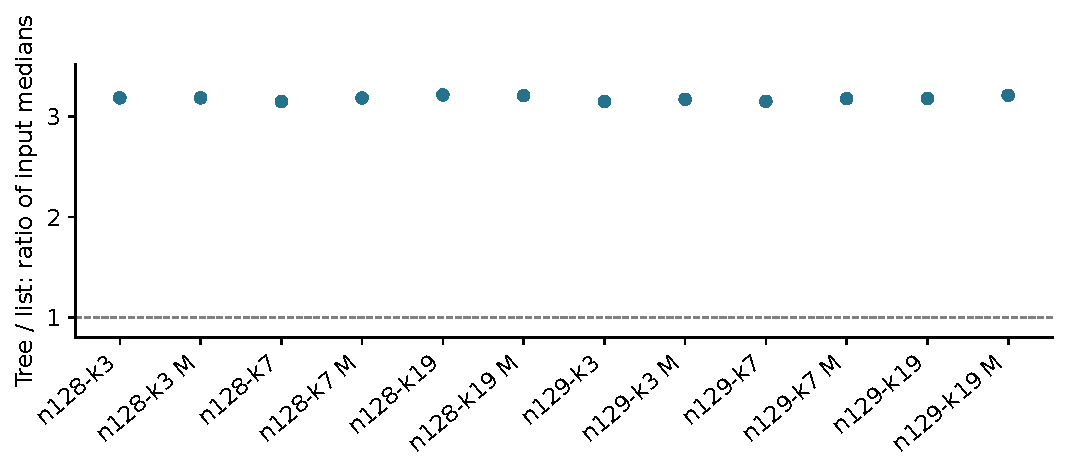
\includegraphics[width=.86\textwidth]{current_formal_targeted.pdf}
\caption{All targeted-set input ratios. M denotes the mirrored construction. Points are ratios of twenty-batch medians, not individual samples or independent random draws.}
\label{fig:results-targeted}
\end{figure}

Ratios range from 3.147 to 3.213; the median is 3.180, with cross-input
quartiles 3.165 and 3.189. The tree is slower on all twelve cases. The absence
of a monotonic relation with $k$ does not disprove a smaller-side bound: these
are complete sorting calls with many other operations, not isolated split
latencies. The small targeted set establishes execution of the intended path
and a bounded whole-call comparison, not its general performance distribution.

\section{Variability and Measurement Accounting}
\label{sec:results-variability}
\label{sec:results-elapsed}

For each input/backend, relative IQR is the R7-interpolated IQR divided by
its own twenty-batch median. Across the common set its median is 1.37\% for
the list and 1.08\% for the tree; maxima are 50.26\% and 61.81\%, respectively.
The targeted-set medians are 1.18\% and 1.55\%, with maxima 9.08\% and 7.52\%.
Thus typical cells have narrow central spreads, but some common-set cells do
not. Every batch is retained, including the high-variability cells. The later
wrapper diagnostic does not identify the cause of those formal-run variations.

One common-set sample batch is below 10 ms; none in the targeted set is.
The frozen calibration criterion was the median of three calibration batches,
not a lower bound on every later batch. B was therefore neither increased nor
reselected, and the observation was not excluded. A fixed batch improves clock
granularity without guaranteeing stability or statistical precision.

Summed sample intervals are 183.511 seconds for the common set and 21.290
seconds for the targeted set. These are accumulated timed intervals, not
campaign wall times: worker startup, GC preparation, validation, compression,
synchronization and other orchestration occur outside them. The recorded
campaigns remain separate, and their absolute times are not pooled with the
older pilot or historical experiments.

\section{Post-Review Access-Hook Diagnostic}
\label{sec:results-hooks}

A separate October 20 diagnostic uses the reviewer's fixed fifteen common-set
inputs at $n=128,512,513$, on the same M4 and CPython 3.12.14 in a later session.
Each input has four isolated processes: list, measured tree, tree without
field-access hooks, and additionally unwrapped operation/phase methods.
Only process-local class attributes change; production files remain frozen.
Three warm-ups precede fifteen batches of 25 calls at 128 or 7 calls at
512/513. All 11,700 timed outputs and 180 warm-up outputs are saved and checked;
the timer includes output append but excludes comparisons and pre-batch GC.
This diagnostic uses its own protocol, not the formal B table or sample count.

\begin{table}[htbp]
\centering
\caption{All fifteen local diagnostic inputs. T, H and U are the measured,
hook-free and additionally unwrapped trees; L is the list. Each row gives
ratios of that input's batch medians. Drop is $100(1-H/T)$, not an additive
cost attribution. Original and mirror constructions are related inputs.}
\label{tab:results-hooks}
\begin{tabular}{rllrrrr}
\toprule
$n$ & Workload & Direction & T/L & H/L & U/L & Drop (\%)\\
\midrule
128 & Low & Original & 3.255 & 1.635 & 1.469 & 49.8\\
128 & Medium & Original & 2.923 & 1.495 & 1.341 & 48.9\\
128 & Heavy & Original & 1.859 & 1.138 & 1.011 & 38.8\\
128 & Heavy & Mirror & 1.890 & 1.135 & 1.014 & 40.0\\
128 & Strict-flat & Original & 3.512 & 1.684 & 1.505 & 52.1\\
512 & Low & Original & 2.600 & 1.298 & 1.153 & 50.1\\
512 & Medium & Original & 2.109 & 1.107 & 0.964 & 47.5\\
512 & Heavy & Original & 1.112 & 0.689 & 0.623 & 38.0\\
512 & Heavy & Mirror & 1.118 & 0.693 & 0.612 & 38.0\\
512 & Strict-flat & Original & 3.086 & 1.487 & 1.305 & 51.8\\
513 & Low & Original & 2.556 & 1.262 & 1.123 & 50.6\\
513 & Medium & Original & 2.102 & 1.088 & 0.977 & 48.3\\
513 & Heavy & Original & 1.103 & 0.687 & 0.615 & 37.7\\
513 & Heavy & Mirror & 1.115 & 0.689 & 0.616 & 38.2\\
513 & Strict-flat & Original & 3.073 & 1.485 & 1.293 & 51.7\\
\bottomrule
\end{tabular}
\end{table}

Removing hooks lowers the tree median by 37.7--52.1\% across the fifteen cases.
Four of fifteen cases, the large heavy constructions, favor the hook-free
tree; the remaining eleven take 1.09--1.68 times the list time.
The diagnostic therefore shows a configuration effect without establishing
a general tree advantage. The diagnostic does not
qualify these modified variants as production backends or isolate an exact
additive overhead share; order and environment limits remain in
\cref{sec:limitations-timing-scopes}.

\clearpage
\section{Historical Rollback-Enabled Evidence}
\label{sec:results-historical}
\label{sec:results-replication}
\label{sec:results-exploratory}

The earlier rollback-enabled study contains 3,600 measured calls on 60
inputs at its own source and environment. Python sort had the smallest
median call time at every historical size. Its paper/reference ratios and
counter correlations compare different pipeline scopes, not the two current
backends. Full tables remain in the unchanged archive indexed in
\cref{sec:appendix-history}; none enters the current numerical tables.

\section{Interpretation Boundary}
\label{sec:results-boundary}

The current comparison supports a clear practical conclusion for the frozen
inputs and this environment: the measured tree configuration with retained access hooks has higher
per-input medians despite its
reviewed source-level amortized bound. Differing object access, wrappers,
local checks, allocation and tree maintenance all contribute to the concrete
programs; the formal experiment does not isolate their individual costs or evaluate
a version with the hooks removed. The data
neither refute that structural bound nor demonstrate a practical linear-time
speed advantage. Broader performance scales and split patterns remain outside
the formal comparison. No causal rollback-removal claim is made.
